\documentclass[border=12pt,tikz]{standalone}
\usepackage{helvet}
\renewcommand{\familydefault}{\sfdefault}
\usepackage{amsmath}
\usepackage{tikz}
\usepackage{tikz-3dplot}
\usetikzlibrary{calc,positioning,shapes.geometric,arrows.meta,decorations.pathreplacing,backgrounds}

% Volume Palette Colors
\definecolor{emeraldpine}{HTML}{1A4D3E}
\definecolor{harvardcrimson}{HTML}{A51C30}
\definecolor{ethdarkblue}{HTML}{1F407A}
\definecolor{ethpetrol}{HTML}{007A87}
\definecolor{ethbronze}{HTML}{B87333}
\definecolor{ink}{HTML}{1A202C}
\definecolor{softink}{HTML}{4A5568}
\definecolor{paleink}{HTML}{CBD5E1}
\definecolor{cardbg}{HTML}{F8FAFC}
\definecolor{shadecolor}{HTML}{F1F5F9}

\begin{document}
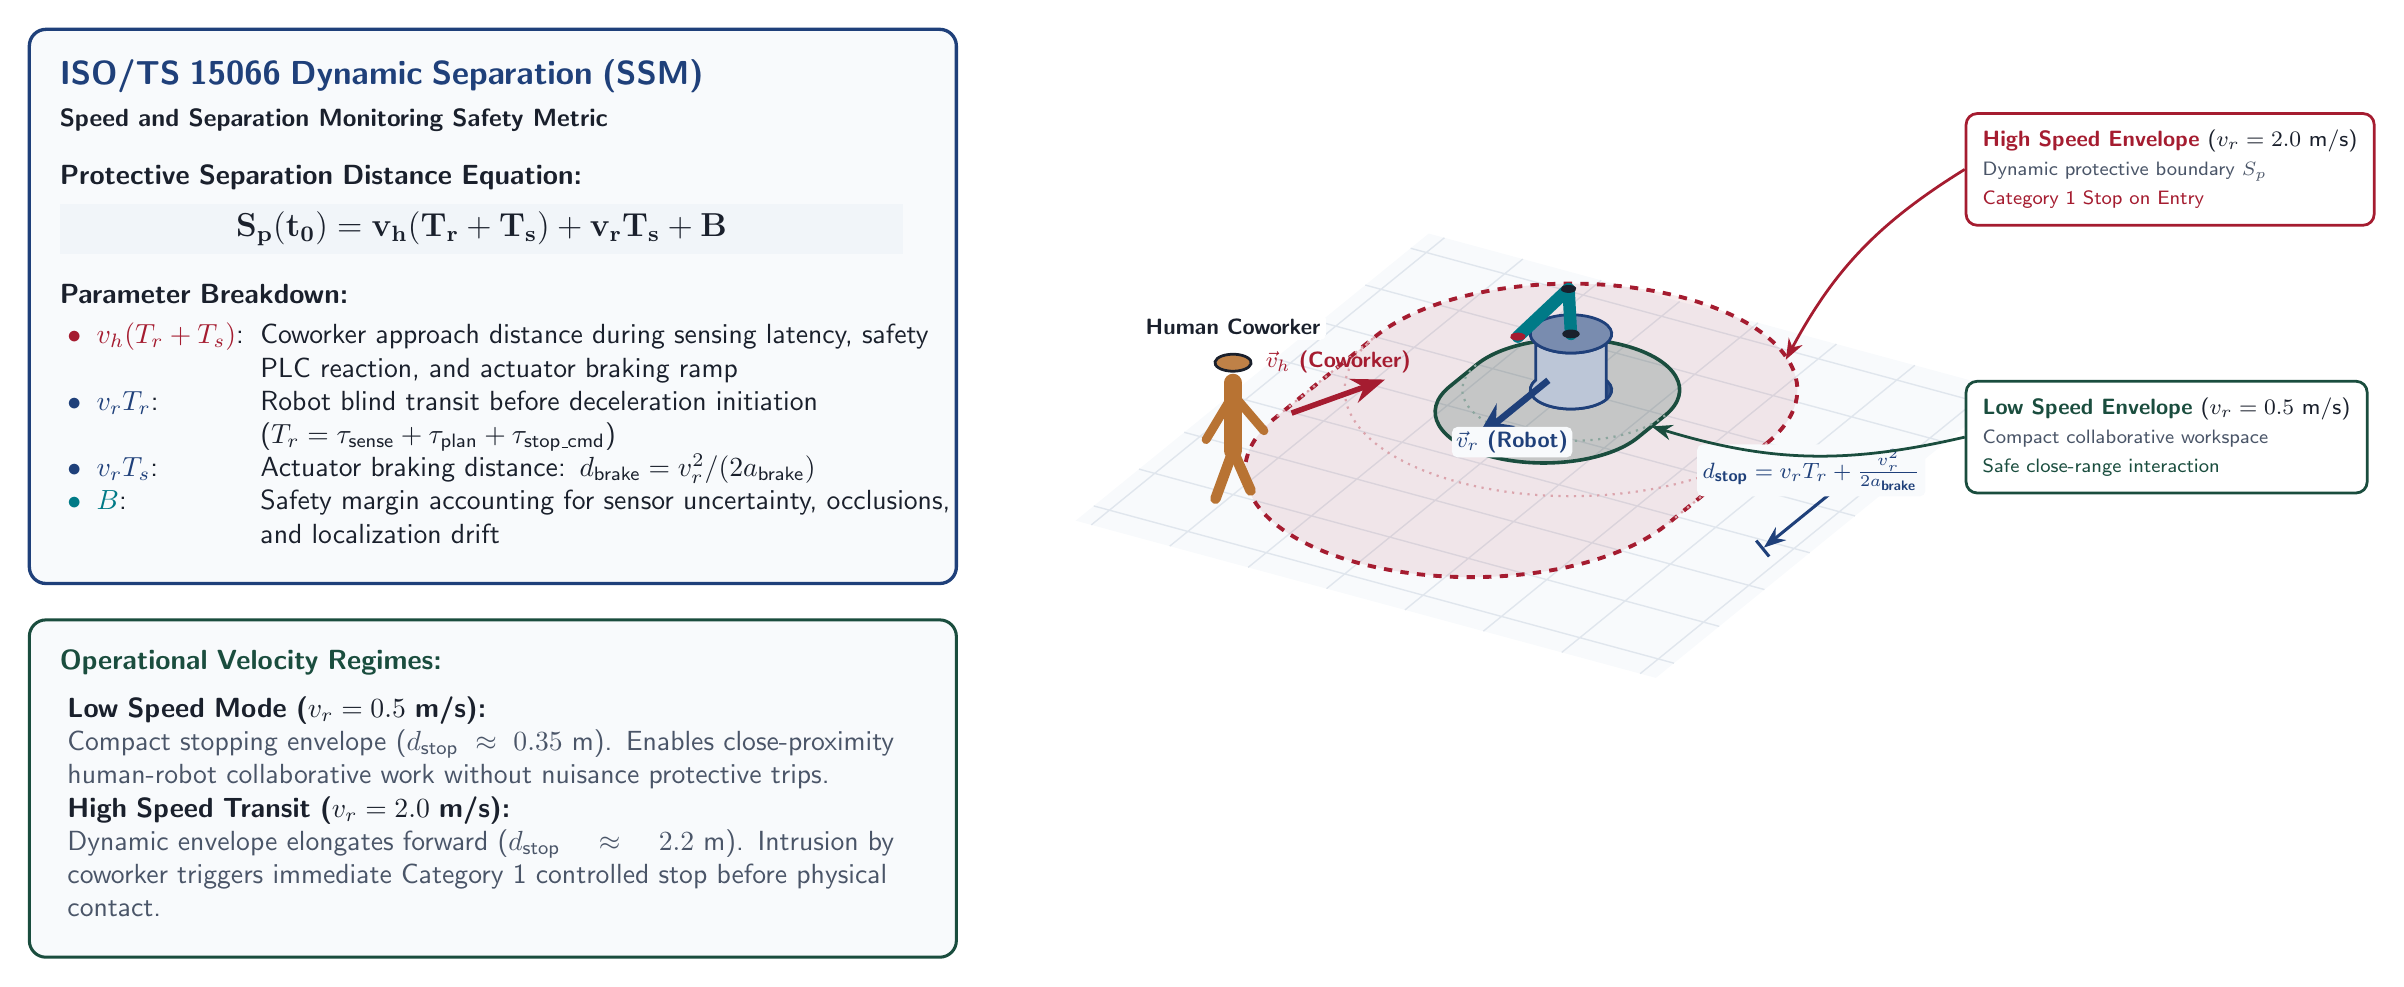
\begin{tikzpicture}[font=\sffamily, >=Stealth]
    
    % ==========================================================
    % LEFT COLUMN: THEORY & SPECIFICATION CARDS (2D canvas)
    % ==========================================================
    \node[anchor=north west, fill=cardbg, draw=ethdarkblue, line width=1.2pt, rounded corners=6pt, inner sep=11pt, text=ink, text width=11.0cm] (theoryCard) at (0, 0) {
        {\large\bfseries\textcolor{ethdarkblue}{ISO/TS 15066 Dynamic Separation (SSM)}}\\[3pt]
        {\small\bfseries Speed and Separation Monitoring Safety Metric}\\[9pt]
        \textbf{Protective Separation Distance Equation:}\\[4pt]
        \colorbox{shadecolor}{\parbox{10.5cm}{\centering\large $\mathbf{S_p(t_0) = v_h (T_r + T_s) + v_r T_s + B}$}}\\[10pt]
        {\bfseries Parameter Breakdown:}\\[5pt]
        \begin{tabular}{@{\;}l@{\hspace{6pt}}p{8.8cm}@{}}
        \textcolor{harvardcrimson}{$\bullet$\;\;$v_h(T_r + T_s)$}: & Coworker approach distance during sensing latency, safety PLC reaction, and actuator braking ramp \\
        \textcolor{ethdarkblue}{$\bullet$\;\;$v_r T_r$}: & Robot blind transit before deceleration initiation ($T_r = \tau_{\text{sense}} + \tau_{\text{plan}} + \tau_{\text{stop\_cmd}}$) \\
        \textcolor{ethdarkblue}{$\bullet$\;\;$v_r T_s$}: & Actuator braking distance: $d_{\text{brake}} = v_r^2 / (2a_{\text{brake}})$ \\
        \textcolor{ethpetrol}{$\bullet$\;\;$B$}: & Safety margin accounting for sensor uncertainty, occlusions, and localization drift
        \end{tabular}
    };

    \node[anchor=north west, fill=cardbg, draw=emeraldpine, line width=1.1pt, rounded corners=6pt, inner sep=11pt, text=ink, text width=11.0cm, below=12pt of theoryCard] (modesCard) {
        {\bfseries\textcolor{emeraldpine}{Operational Velocity Regimes:}}\\[6pt]
        \begin{tabular}{@{\;}p{10.5cm}@{}}
        \textbf{Low Speed Mode ($v_r = 0.5$ m/s):}\newline
        \textcolor{softink}{Compact stopping envelope ($d_{\text{stop}} \approx 0.35$ m). Enables close-proximity human-robot collaborative work without nuisance protective trips.}\\[6pt]
        \textbf{High Speed Transit ($v_r = 2.0$ m/s):}\newline
        \textcolor{softink}{Dynamic envelope elongates forward ($d_{\text{stop}} \approx 2.2$ m). Intrusion by coworker triggers immediate Category 1 controlled stop before physical contact.}
        \end{tabular}
    };

    % ==========================================================
    % CENTER: 3D ISOMETRIC ENVELOPE VISUALIZATION
    % ==========================================================
    \tdplotsetmaincoords{62}{120}
    \begin{scope}[shift={(19.6, -4.6)}, scale=1.15, tdplot_main_coords]
        
        % 1. FLOOR GRID
        \begin{scope}[canvas is xy plane at z=0]
            \fill[cardbg] (-2.4, -3.2) rectangle (5.4, 4.2);
            \draw[step=1cm, paleink!60, line width=0.5pt] (-2.4, -3.2) grid (5.4, 4.2);
            
            % High Speed Dynamic Envelope (v_r = 2.0 m/s) - Crimson
            \fill[harvardcrimson, fill opacity=0.09] 
                (0, 2.5) arc (90:270:2.5) -- (2.2, -2.5) arc (270:450:2.5) -- cycle;
            \draw[harvardcrimson, line width=1.4pt, dashed] 
                (0, 2.5) arc (90:270:2.5) -- (2.2, -2.5) arc (270:450:2.5) -- cycle;
                
            % Standstill circular boundary projection
            \draw[harvardcrimson!40, line width=0.8pt, dotted] (0, 2.5) arc (90:-90:2.5);
            \draw[harvardcrimson!40, line width=0.8pt, dotted] (0, 2.5) -- (2.2, 2.5);
            \draw[harvardcrimson!40, line width=0.8pt, dotted] (0, -2.5) -- (2.2, -2.5);

            % Low Speed Dynamic Envelope (v_r = 0.5 m/s) - Emerald
            \fill[emeraldpine, fill opacity=0.20] 
                (0, 1.2) arc (90:270:1.2) -- (0.6, -1.2) arc (270:450:1.2) -- cycle;
            \draw[emeraldpine, line width=1.3pt] 
                (0, 1.2) arc (90:270:1.2) -- (0.6, -1.2) arc (270:450:1.2) -- cycle;
            \draw[emeraldpine!50, line width=0.8pt, dotted] (0, 1.2) arc (90:-90:1.2);

            % Dynamic expansion dimension line (clean clearance at Y = 3.7)
            \draw[|<->|, line width=1.1pt, ethdarkblue] (0, 3.7) -- (2.2, 3.7) 
                node[midway, above=4pt, fill=cardbg, inner sep=2pt, rounded corners=2pt, font=\bfseries\footnotesize, text=ethdarkblue, sloped] 
                {$d_{\text{stop}} = v_r T_r + \frac{v_r^2}{2a_{\text{brake}}}$};
        \end{scope}

        % 2. ROBOT MODEL (Base cylinder + Articulated Arm)
        \begin{scope}[shift={(0,0,0)}]
            \tdplotdrawarc[fill=ethdarkblue!90, draw=ethdarkblue, line width=1pt]{(0,0,0)}{0.45}{0}{360}{}{}
            \draw[ethdarkblue, line width=1pt, fill=ethdarkblue!30] 
                (0,-0.45,0) -- (0,-0.45,0.7) arc (-90:90:0.45) -- (0,0.45,0) arc (90:-90:0.45) -- cycle;
            \tdplotdrawarc[fill=ethdarkblue!60, draw=ethdarkblue, line width=1pt]{(0,0,0.7)}{0.45}{0}{360}{}{}
            
            % Manipulator arm
            \draw[ethpetrol, line width=4.5pt, line cap=round, line join=round] 
                (0,0,0.7) -- (0.4, 0.2, 1.5) -- (1.0, -0.1, 1.1);
            \filldraw[ink] (0,0,0.7) circle (0.09);
            \filldraw[ink] (0.4, 0.2, 1.5) circle (0.08);
            \filldraw[harvardcrimson] (1.0, -0.1, 1.1) circle (0.08);
        \end{scope}

        % Robot Velocity Vector (pointing forward in +X)
        \draw[->, line width=2.4pt, ethdarkblue] (0.5, 0, 0.35) -- (2.1, 0, 0.35) 
            node[midway, below=5pt, fill=cardbg, inner sep=1.5pt, rounded corners=2pt, font=\bfseries\footnotesize, text=ethdarkblue] {$\vec{v}_r$ (Robot)};

        % 3. HUMAN COWORKER MODEL at (4.0, -2.0, 0)
        \begin{scope}[shift={(4.0, -2.0, 0)}]
            \draw[ethbronze, line width=6.5pt, line cap=round] (0,0,0.55) -- (0,0,1.4);
            \draw[ethbronze, line width=3.8pt, line cap=round] (0,0,0.55) -- (-0.18, 0.12, 0);
            \draw[ethbronze, line width=3.8pt, line cap=round] (0,0,0.55) -- (0.18, -0.12, 0);
            \draw[ethbronze, line width=3.2pt, line cap=round] (0,0,1.25) -- (-0.25, 0.25, 0.75);
            \draw[ethbronze, line width=3.2pt, line cap=round] (0,0,1.25) -- (0.25, -0.2, 0.75);
            \filldraw[ethbronze!90, draw=ink, line width=1pt] (0,0,1.65) circle (0.2);
        \end{scope}

        % Human approach vector
        \draw[->, line width=2pt, harvardcrimson] (3.4, -1.6, 0.85) -- (2.2, -1.1, 0.85) 
            node[midway, above=4pt, font=\bfseries\footnotesize, text=harvardcrimson] {$\vec{v}_h$ (Coworker)};
        \node[font=\bfseries\footnotesize, text=ink, fill=white, inner sep=2pt, rounded corners=2pt] 
            at (4.0, -2.0, 2.1) {Human Coworker};

        % Callout anchor coordinates
        \coordinate (lowCalloutTarget) at (0.3, 1.2, 0);
        \coordinate (highCalloutTarget) at (-1.8, 1.7, 0);
    \end{scope}

    % ==========================================================
    % RIGHT COLUMN: STACKED CALLOUT CARDS (2D coordinates)
    % ==========================================================
    % High speed envelope callout (top right)
    \node[anchor=west, fill=white, draw=harvardcrimson, line width=1pt, rounded corners=4pt, inner sep=6pt, font=\footnotesize, text=ink, align=left] 
        (calloutHigh) at (24.6, -1.8) {
            \textcolor{harvardcrimson}{\bfseries High Speed Envelope} ($v_r = 2.0\text{ m/s}$)\\[1pt]
            \textcolor{softink}{\scriptsize Dynamic protective boundary $S_p$}\\[1pt]
            \textcolor{harvardcrimson}{\scriptsize Category 1 Stop on Entry}
        };
    \draw[->, line width=1pt, harvardcrimson] (calloutHigh.west) to[bend right=15] (highCalloutTarget);

    % Low speed envelope callout (bottom right, neatly stacked)
    \node[anchor=west, fill=white, draw=emeraldpine, line width=1pt, rounded corners=4pt, inner sep=6pt, font=\footnotesize, text=ink, align=left] 
        (calloutLow) at (24.6, -5.2) {
            \textcolor{emeraldpine}{\bfseries Low Speed Envelope} ($v_r = 0.5\text{ m/s}$)\\[1pt]
            \textcolor{softink}{\scriptsize Compact collaborative workspace}\\[1pt]
            \textcolor{emeraldpine}{\scriptsize Safe close-range interaction}
        };
    \draw[->, line width=1pt, emeraldpine] (calloutLow.west) to[bend left=15] (lowCalloutTarget);

\end{tikzpicture}
\end{document}
